\section*{Union-find implementation%
\TAGS{union-find}}

Union find's equivalence graphs can be represented with arrays: the
indices corresponding to non-canonical representatives store the
element that their directed edge in the equivalence graph points
to. Canonical representatives can store their own index, but in order
to efficiently implement union-find, it's useful for canonical
representatives to store a negative number, the absolute value of
which is the maximum height of any path to that canonical
representative.


\checkpoint*{\TAGS{union-find}}

For the following series of union operations, make the \emph{worst
  possible} decision at every step when you connect canonical
representatives to try to make the paths as long as possible. Draw the
state of the array after every step. How long is the longest path?
\begin{center}
  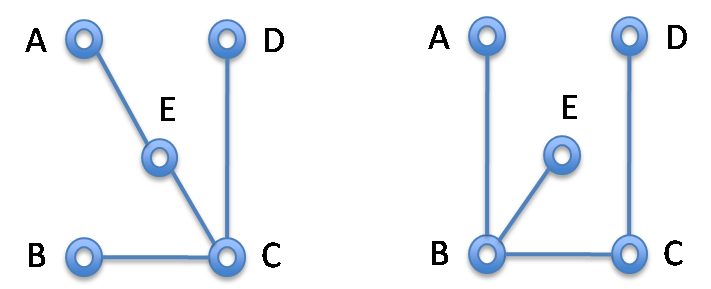
\includegraphics[width=.75\textwidth]{\img/graph2.png}
\vspace{-1ex}
\end{center}

\begin{solution}
  There are many answers. All should have edges from either 1 or 2
  leading to 3, and an edge from 3 to 4: the longest path should be
  5. Here's one example.
\begin{center}
  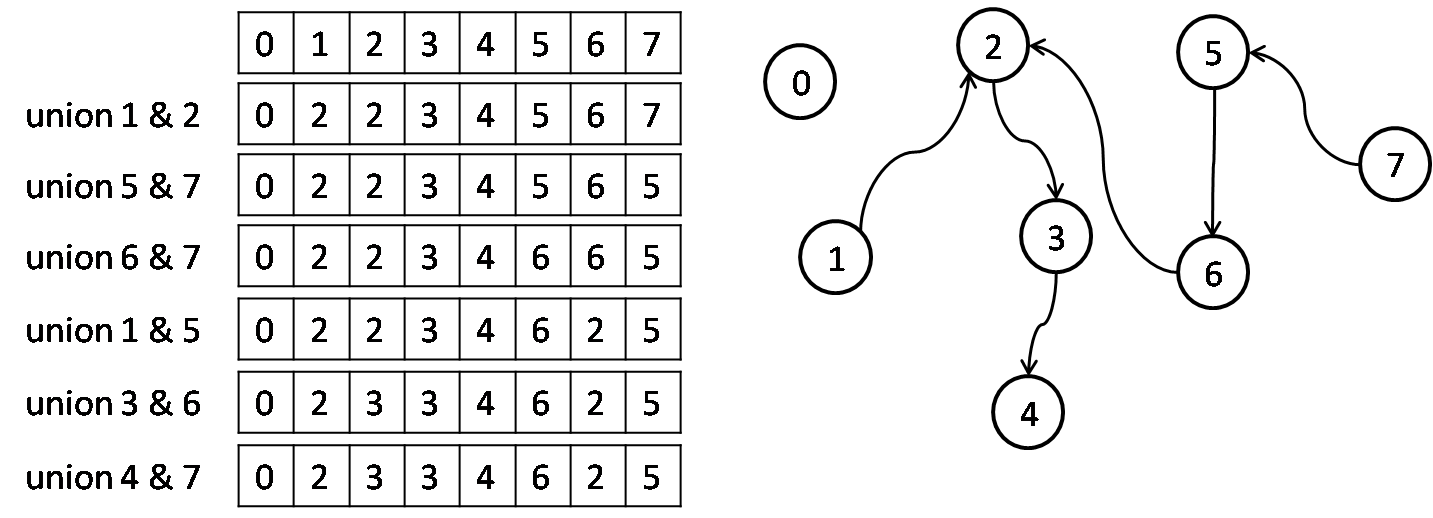
\includegraphics[width=.75\textwidth]{\img/graph2-sol.png}
\end{center}
\end{solution}


\checkpoint*{\TAGS{union-find}}

Describe a series of unions that could lead to this equivalence graph:
\begin{center}
  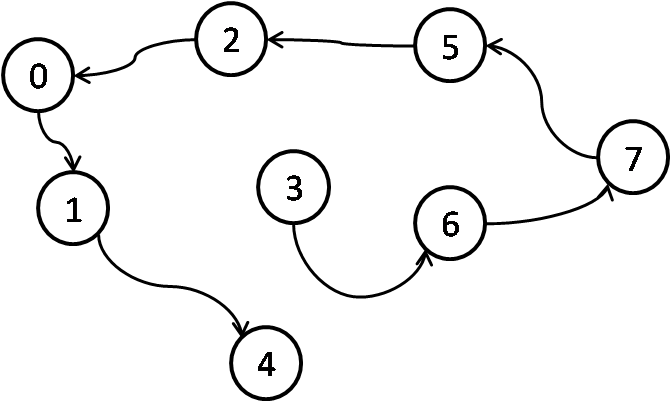
\includegraphics[width=.3\textwidth]{\img/graph4.png}
\vspace{-6ex}
\end{center}
\begin{solution}\par
Union 3 and 6\\
Union one of \{3,6\} and 7\\
Union one of \{3,6,7\} and 5\\
Union one of \{3,6,7,5\} and 2\\
Union one of \{3,6,7,5,2\} and 0 \ldots
\end{solution}

\checkpoint*{\TAGS{union-find}}

If we use the tree-height storing version of union find on the unions
from the last checkpoint, what happens?
\begin{center}
\vspace{-2ex}
  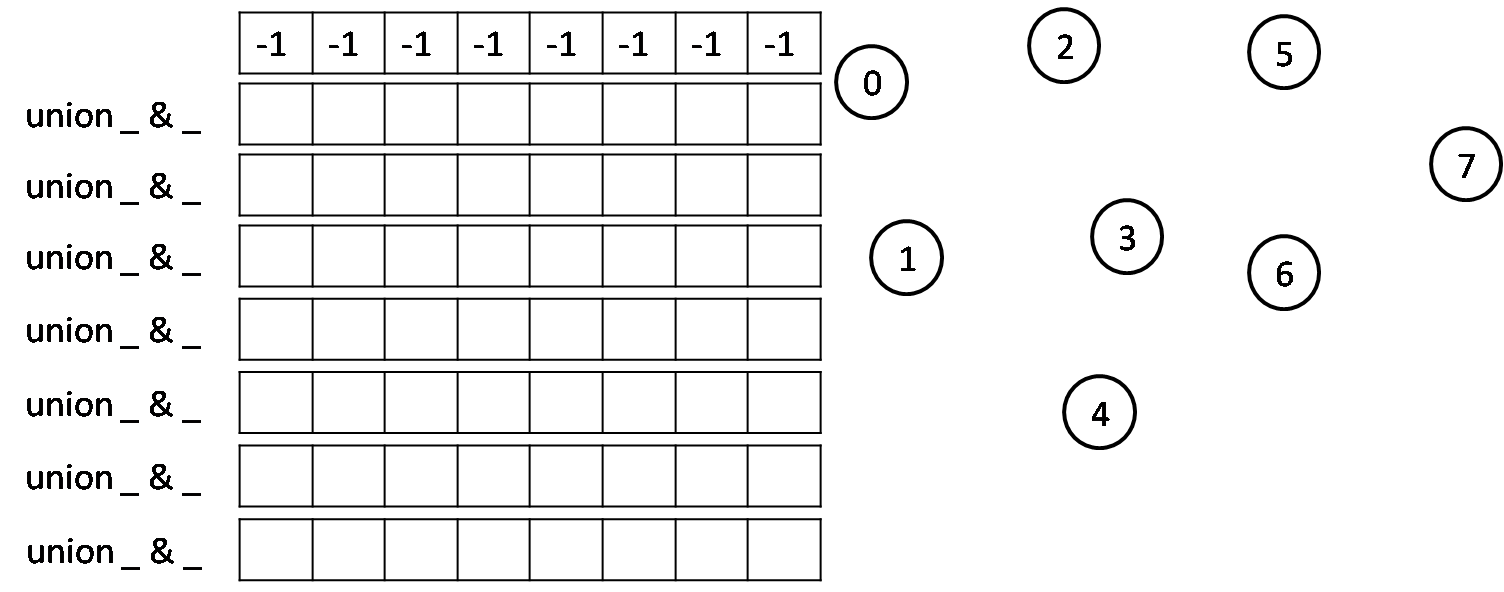
\includegraphics[width=.75\textwidth]{\img/graph3.png}
\vspace{-1ex}
\end{center}

\begin{solution}
  Either everything points to 3 or everything points to 6, and the
  canonical representative stores -2.
\end{solution}

\checkpoint*{\TAGS{union-find}}
If we use the tree-height storing version of union-find, what's a worst-case
equivalence graph? What's a series of union operations that would create it?

\begin{solution}
  In the worst case, there will be exactly one path with length $3 =
  \log_2 8$.
\end{solution}
